%------------------------------------------------
%	PACKAGES AND DOCUMENT CONFIGURATIONS
%------------------------------------------------
\documentclass[11pt]{article}
\usepackage{amsmath} % Required for some math elements
\usepackage{hyperref} 
\usepackage{xcolor}
\usepackage{lipsum} 
\usepackage{cite}
\usepackage{graphicx} % Required for the inclusion of images
\usepackage{algorithmic}
\usepackage{array}
\usepackage{bookmark}
\usepackage{listings}
\usepackage{amssymb}
\usepackage{enumitem}
\usepackage{pythonhighlight}
\usepackage[T1]{fontenc}
\usepackage{inconsolata}
\usepackage[margin=16mm]{geometry}
\usepackage[caption=false, font=footnotesize]{subfig}
\usepackage[active,tightpage]{preview}

\renewcommand{\PreviewBorder}{1in}
\newcommand{\Newpage}{\end{preview}\begin{preview}}

\newlist{steps}{enumerate}{1}
\setlist[steps, 1]{label = Step \arabic*:}

\hypersetup{ %color attributes of citation, link, etc.
    colorlinks=true,
    linkcolor=blue,
    filecolor=gray,      
    urlcolor=blue,
    citecolor=blue,
}

\newcommand{\matlab}{\textsc{Matlab }} %very important and totally necessary addition

\newcommand\Item[1][]{%
  \ifx\relax#1\relax  \item \else \item[#1] \fi
  \abovedisplayskip=0pt\abovedisplayshortskip=0pt~\vspace*{-\baselineskip}}

%----------------------------------
%	DOCUMENT INFORMATION
%----------------------------------
 
\title{ECEN321 : Hypothesis Testing \\ Lab 4 Submission}
\author{Daniel Eisen : 300447549}
\date{\today}

\begin{document}
\begin{preview}
\maketitle
%-----------------------------
%	DOCUMENT CONTENT
%-----------------------------
\section{Introduction}

\section{Theory}

\section{Results}
A python script was implemented to generate a Poisson distributed random variable from a random uniform disruption and then evaluated using the $\chi^2$ test.

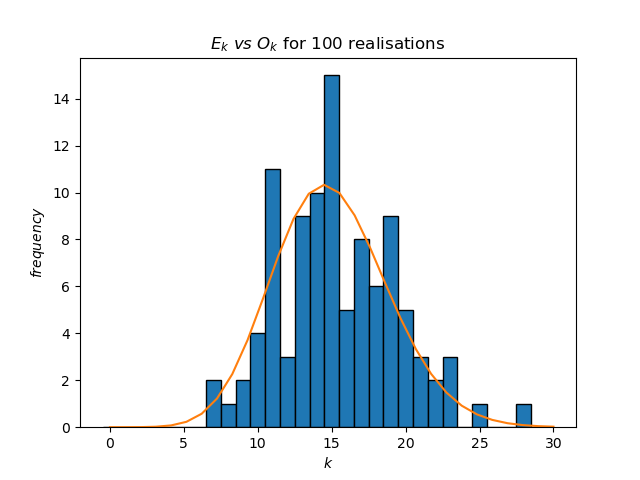
\includegraphics[width=0.3\textwidth]{inc/100.png}
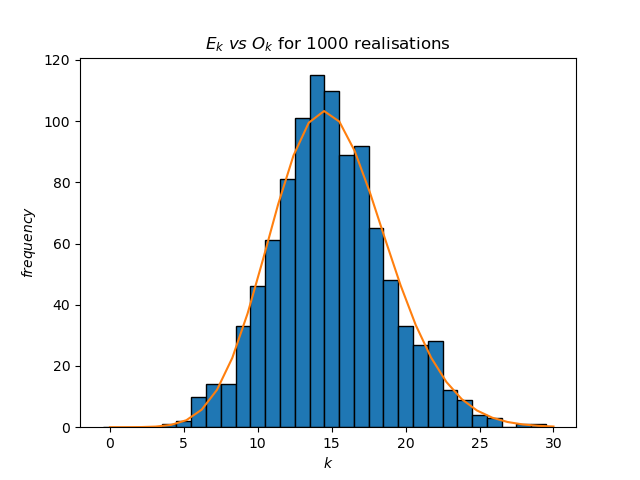
\includegraphics[width=0.3\textwidth]{inc/1000.png}
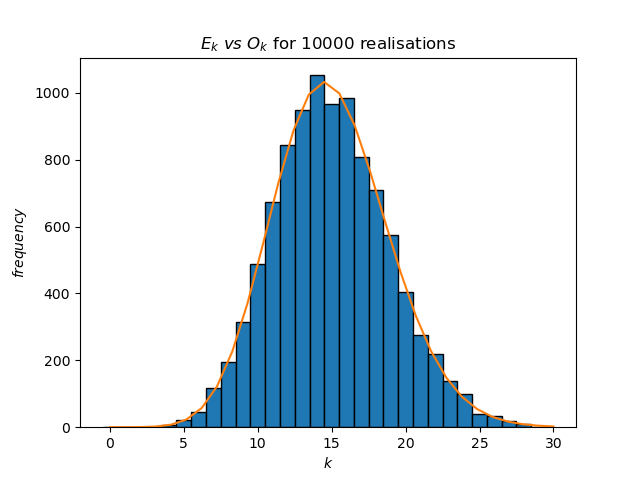
\includegraphics[width=0.3\textwidth]{inc/10000.png}
\begin{center}
        Figure 1.
\end{center}

Figure 1 show three runs of


When N become around 1000-1400 the critical value drops below 0.99 half the time. 

\Newpage
\section*{Appendix}
\subsection*{Part 1}
\inputpython{../py/lab4.py}{1}{60}

\end{preview}
\end{document}